\begin{question}
\noindent Shape $M$ (a mission-control observation panel, shaped as a triangle) is rotated to give shape $N$, as shown on the grid.

\begin{center}
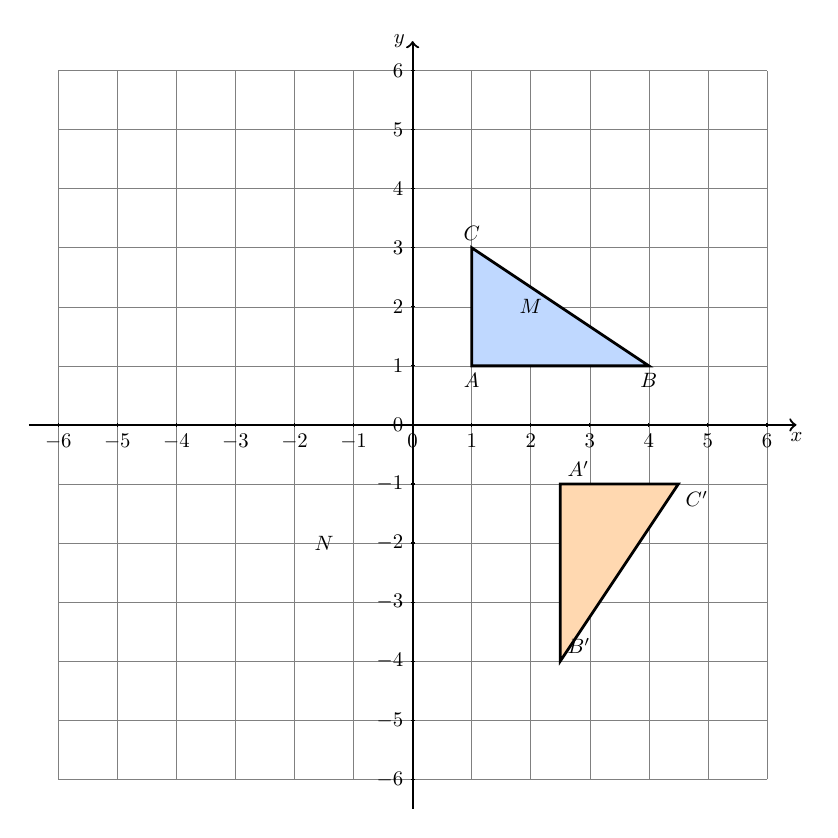
\begin{tikzpicture}[scale=0.75, transform shape]
    \def\axisLimit{6}

    \definecolor{borderColour}{HTML}{000000}
    \definecolor{fillColourM}{HTML}{BFD8FF}
    \definecolor{fillColourN}{HTML}{FFD8B0}

    % Draw grid
    \draw[step=1cm,gray,very thin] (-\axisLimit,-\axisLimit) grid (\axisLimit,\axisLimit);

    % Draw axes
    \draw[thick,->] (-\axisLimit-0.5,0) -- (\axisLimit+0.5,0) node[anchor=north] {$x$};
    \draw[thick,->] (0,-\axisLimit-0.5) -- (0,\axisLimit+0.5) node[anchor=east] {$y$};

    % Label x-axis and y-axis
    \foreach \x in {-\axisLimit,...,\axisLimit}
        \draw (\x cm,1pt) -- (\x cm,-1pt) node[anchor=north] {$\x$};
    \foreach \y in {-\axisLimit,...,\axisLimit}
        \draw (1pt,\y cm) -- (-1pt,\y cm) node[anchor=east] {$\y$};

    % Shape M: A(1,1), B(4,1), C(1,3)
    \coordinate (A) at (1,1);
    \coordinate (B) at (4,1);
    \coordinate (C) at (1,3);
    \filldraw[fill=fillColourM, draw=borderColour, line width=1pt] (A) -- (B) -- (C) -- cycle;
    \node[below] at (A) {$A$};
    \node[below] at (B) {$B$};
    \node[above] at (C) {$C$};
    \node at (2,2) {$M$};

    % Centre of rotation at (1,-1)
    \coordinate (centre) at (1,-1);

    % Shape N: rotate M by 90 degrees clockwise (i.e. -90) about (1,-1)
    \coordinate (Ap) at ([rotate around={-90:(centre)}]A);
    \coordinate (Bp) at ([rotate around={-90:(centre)}]B);
    \coordinate (Cp) at ([rotate around={-90:(centre)}]C);
    \filldraw[fill=fillColourN, draw=borderColour, line width=1pt] (Ap) -- (Bp) -- (Cp) -- cycle;
    \node[above right] at (Ap) {$A'$};
    \node[above right] at (Bp) {$B'$};
    \node[below right] at (Cp) {$C'$};
    \node at (-1.5,-2) {$N$};

\end{tikzpicture}
\end{center}

\noindent Describe fully the single transformation that maps shape $M$ onto shape $N$.

\vspace{5cm}

\begin{flushright}
    \answerlines{3}{3}
\end{flushright}
\end{question}